\documentclass[11pt,a4paper]{article}
\usepackage[utf8]{inputenc}
\usepackage{graphicx}
\usepackage{url}
\usepackage{xspace}
\usepackage{amsmath}
\usepackage{hyperref}
\usepackage[usenames,dvipsnames]{color}
\usepackage{listings}
\newcommand{\CodeSymbol}[1]{\textcolor{Bittersweet}{#1}}
\lstset{
   language=Ada,
   keywordstyle=\color{RedViolet}\ttfamily\bf,
   showspaces=false,
   basicstyle={\scriptsize \sffamily},
   commentstyle=\color{red}\textit,
   stringstyle=\color{MidnightBlue}\ttfamily,
   string=[b]",  % remove ' from string delimiter as it interfers with attributes
   showtabs=false,
   showstringspaces=false,
   morekeywords=[1]Pre,
   morekeywords=[1]Post,
   morekeywords=[1]Test\_Case,
   morekeywords=[1]Contract\_Cases,
   morekeywords=[1]some,
   morekeywords=[1]Old,
   morekeywords=[1]Global,
   morekeywords=[1]Depends,
   morekeywords=[1]Loop\_Invariant,
   morekeywords=[1]Loop\_Variant,
   morekeywords=[1]Loop\_Entry,
   morekeywords=[1]Increases,
   literate={(}{{\CodeSymbol{(}}}1
            {)}{{\CodeSymbol{)}}}1
            {>}{{\CodeSymbol{$>$}}}1
            {>=}{{\CodeSymbol{$\ge$}}}1
            {<}{{\CodeSymbol{$<$}}}1
            {<=}{{\CodeSymbol{$\le$}}}1
            {=}{{\CodeSymbol{$=$}}}1
            {:}{{\CodeSymbol{$:$}}}1
            {.}{{\CodeSymbol{$.$}}}1
            {;}{{\CodeSymbol{$;$}}}1
            {/=}{{\CodeSymbol{$\ne$}}}1
            {=>}{{\CodeSymbol{$\Rightarrow$}}}1
            {->}{{\CodeSymbol{$\rightarrow$}}}1
            {<->}{{\CodeSymbol{$\leftrightarrow$}}}1
}

\newcommand{\DO}{\textsc{do-178}\xspace}
\newcommand{\DOB}{\textsc{do-178b}\xspace}
\newcommand{\DOC}{\textsc{do-178c}\xspace}
\newcommand{\hilite}{Hi-Lite\xspace}
\newcommand{\openetcs}{openETCS\xspace}
\newcommand{\gnatprove}{GNATprove\xspace}
\newcommand{\oldspark}{SPARK~2005\xspace}
\newcommand{\newspark}{SPARK~2014\xspace}
\newcommand{\spark}{SPARK\xspace}
\newcommand{\ada}{Ada\xspace}
\newcommand{\adatwtw}{Ada~2012\xspace}
\newcommand{\altergo}{Alt-Ergo\xspace}

\newcommand{\etc}{\textit{etc.}\xspace}
\newcommand{\ie}{\textit{i.e.}\xspace}
\newcommand{\adhoc}{\textit{ad hoc}\xspace}
\newcommand{\Eg}{\textit{E.g.}\xspace}
\newcommand{\eg}{\textit{e.g.}\xspace}
\newcommand{\etal}{\textit{et al.}\xspace}
\newcommand{\wrt}{w.r.t.\xspace}
\newcommand{\aka}{a.k.a.\xspace}
\newcommand{\resp}{resp.\xspace}

\urlstyle{sf}

\begin{document}

\title{Auto-Active Proof of Red-Black Trees in SPARK}

\author{%
\large Claire Dross and Yannick Moy\\
\normalsize AdaCore, 46 rue d'Amsterdam, F-75009 Paris (France)}

\date{}

\maketitle

\paragraph{Abstract}
SPARK is a subset of the Ada programming language targeted at safety- and
security-critical applications. SPARK formal verification toolset allows to
guarantee that a SPARK program is free from broad classes of errors (like reads
of uninitialized data and run-time errors) and that it complies with its
specification. While the former is a well adopted practice among SPARK users,
the latter is used much more narrowly, owing to the cost of specifying the
behavior of programs and even more the cost of achieving proof of such
specifications. SPARK relies on automatic provers to keep the cost of formal
verification reasonable, and on the techniques of auto-active verification for
interacting with automatic provers. In this paper, we present how we applied
auto-active verification to formally verify a library of red-black trees. To
the best of our knowledge, this is the most advanced use of auto-active
verification so far.

\paragraph{Keywords}
System formal development, Verification and validation,
Certification and dependability

\section{Introduction}

\section{Preliminaries}
\subsection{SPARK 2014}

SPARK is a subset of the Ada programming language targeted at safety-
and security-critical applications. SPARK builds on the strengths of
Ada for creating highly reliable and long-lived software. SPARK
restrictions ensure that the behavior of a SPARK program is
unambiguously defined, and simple enough that formal verification
tools can perform an automatic diagnosis of conformance between a
program specification and its implementation. The SPARK language and
toolset for formal verification has been applied over many years to
on-board aircraft systems, control systems, cryptographic systems, and
rail systems~\cite{sparkbook2012,oneill2012}.

In the versions of SPARK up to SPARK 2005, specifications are written as
special annotations in comments. Since version SPARK 2014~\cite{sparkERTS2014},
specifications are written as special Ada constructs attached to
declarations. In particular, various contracts can be attached to subprograms:
data flow contracts (introduced by \texttt{global}), information flow contracts,
and functional contracts (preconditions and postconditions, introduced
respectively by \texttt{pre} and \texttt{post}). An important difference
between SPARK 2005 and SPARK 2014 is that functional contracts are executable in
SPARK 2014, which greatly facilitates the combination between test and proof
(see Section~\ref{sec:test-and-proof}). The definition of the language subset
is motivated by the simplicity and feasability of formal analysis and the need
for an unambiguous semantics. Tools are available that provide flow analysis
and proof of SPARK programs.

Flow analysis checks correct access to data in the program: correct access to
global variables (as specified in data and information flow contracts) and
correct access to initialized data. Proof is used to demonstrate that the
program is free from run-time errors such as arithmetic overflow, buffer
overflow and division-by-zero, and that the functional contracts are correctly
implemented.

\subsection{Auto-active Verification}
\label{sec-prelim-auto-active}

The term \emph{auto-active verification} was coined in 2010 by researcher
Rustan Leino~\cite{Leino10usableauto-active} to designate \textit{tools where
  user input is supplied before VC generation [and] therefore lie between
  automatic and interactive verification} (hence the name auto-active). This is
in contrast to fully automatic verifiers for which \textit{the specification is
  fixed} and interactive verifiers for which \textit{the user input is supplied
  after VC generation, which is the typical case when the reasoning engine is
  an interactive proof assistant}. Auto-active verification is at the center of
the academic formal program verification toolsets Dafny~\cite{Leino2010Dafny},
the Eiffel Verification Environment (EVE)~\cite{Furia2016},
Why3~\cite{filliatre2013Why3} as well as the industrial formal program
verification toolsets Frama-C and SPARK.

In all these toolsets, auto-active verification consists in a set of
specification features at the level of the source language, and a set of tool
capabilities to interact with users at the level of the source code. The
specification features consist at least in constructs to specify function
contracts (preconditions and postconditions) and data invariants, as well as
specialized forms of assertions (loop invariants and loop variants, assumptions
and assertions). All the toolsets mentioned above also support a feature to
instrument code for verification, usually referred to as ghost code. Ghost
functions may be referred to as lemmas when they are used to prove a property
that is used at the point where the function is called. See
\cite{kosmatov:hal-01344110} for a comparison of how ghost code differs between
Why3, Frama-C and SPARK. Various tool capabilities facilitate user interaction
at source level: fast running time that exploits multiprocessor architectures
and minimizes rework between runs, ability to trade running time for more
verification power, feedback from the toolset when verification is unsuccessful
(counterexamples in particular).

Auto-active verification in the above toolsets has been used to fully verify
algorithms, libraries and even complete applications: examples include a
container library in Eiffel~\cite{Polikarpova2015}, distributed systems in
Dafny~\cite{Hawblitzel2015IronFleet}, secure execution of apps in
Dafny~\cite{Hawblitzel2014Ironclad}, binary heaps in Why3~\cite{tafat11rr},
allocators in SPARK~\cite{Dross2016}.

\subsection{Red-Black Trees}

Red-black trees are a kind of self-balancing binary search trees. Nodes in the
tree are colored red or black, and balance is maintained by ensuring that two
properties are preserved: (1) a red node can only have black children, and (2)
every path from the root to a leaf has the same number of black nodes. The
consequence of these two properties is that the path from the root to a leaf
can be at most twice as long as the path from the root to another leaf.

Implementations of red-black trees are used in the Linux kernel (in C) and
standard container libraries for various languages (C++ STL, Java.util,
Ada). The insertion and deletion algorithms work by inserting or deleting the
node as in a binary search tree, which may violate properties (1) and (2)
above, and then restore the balance by working their way up on the path from
the root to the point of insertion or deletion. At every node on this path, the
algorithms may \emph{rotate} the subtree, which consists in a local
rearrangement of nodes to restore properties (1) and (2). These algorithms are
sufficiently complex that no implementation of imperative red-black trees has
been fully verified. See Section~\ref{related-work} for a list of the closest
works, including some using auto-active verification. We are following the
algorithm from Cormen et al.~\cite{Cormen2009} for insertion in a red-black
tree. We did not implement the deletion algorithm.

\section{Red-Black Trees in SPARK}
\subsection{Invariants and Models}
\label{sec-rbt-inv}
% invariants of data structures
% relation between invariants and models
% public model of RBT
% internal model of tree

% hierarchy done with proof in mind, separation of concerns
%    binary_trees => tree structure
%    search_trees => ordered values
%    red_black_trees => balanceness
% properties stored in (private) invariants and reflected in (public) models
%    binary_trees => reachability
%    search_trees => set of contained values
%    red_black_trees => no model
% models should be easy to use/complex to verify to factor complexity
%  ex: provide a model of reachability
% primitives needed by upper levels provided at lower level were they abide by the invariant

Though they are relatively complex data structures, implementing red black trees
correctly is not a challenge as numerous implementations and descriptions of the
algorithm are readily available. However, the algorithm is already complicated
enough for full static verification to require re-designing the
software from the start with proof in mind.
To this aim, we have divided our implementation of red black trees in three
distinct parts, each concerned only with parts of the data structure properties.

The first part defines binary trees. It is only concerned with properties
relative to the tree structure of the underlying memory.
The second part associates values to nodes of binary trees to define search trees.
It is concerned with order of values in the tree.
The third part enforces balancing using the classical red black tree coloring
mechanism.

At each level, the separation of concerns is ensured by the use of type invariants.
As defined by Ada 2012 standard, type invariants are boolean properties associated
with private types which can be temporarily violated in the private functions of the
type but must always hold outside of private scope of the type.
More precisely, the property that should be ensured at each level (tree structure,
order of values, or balancing) is enforced at the boundary of every function
of this level and then assumed in upper levels.

For example, let us look at the invariant of binary trees. Binary trees are
encoded using an imperative data structure as represented in Figure~\ref{fig-binary}.
Each node contains a reference to is right and left child if any as well as a
reference to its parent and a position, which may be Top, for the root, or
Right or Left depending on their position with respect to their parent.

\begin{figure}[ht]
\begin{center}
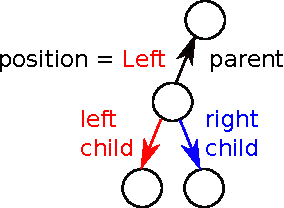
\includegraphics[width=4cm]{tree_structure.pdf}\hfill
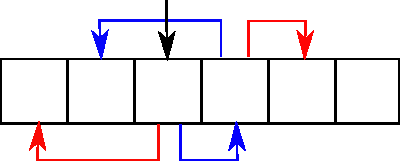
\includegraphics[width=5cm]{binary_1.pdf}\hfill
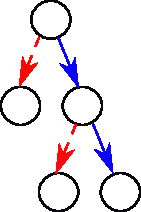
\includegraphics[width=2cm]{binary_2.pdf}
\caption{\label{fig-binary} From left to right: Representation of nodes in binary trees.
Example of a binary tree, for readability, parents and positions are not represented.
The binary tree represented in previous figure.}
\end{center}
\end{figure}

The invariant of binary trees is given in Figure~\ref{fig-binary-inv}.
As can be seen, it is only concerned with low level sanity of the
tree representation.

\begin{figure}[ht]
\begin{small}
\begin{lstlisting}
 --  Cells that are not allocated yet have default values
(for all I in F.S + 1 .. Max => F.C (I) = (Empty, Empty, Empty, Top))

--  Parent and children of all cells are allocated or empty
and then (for all I in Index_Type => F.C (I).Parent in Empty .. F.S)
and then (for all I in Index_Type => F.C (I).Left in Empty .. F.S)
and then (for all I in Index_Type => F.C (I).Right in Empty .. F.S)

--  If a cell is the root of a tree (position Top) it has no parent
and then (for all I in Index_Type =>
           (if F.C (I).Position = Top then F.C (I).Parent = Empty))

--  If a cell I has a left child, then its left child has position
--  Left and parent I.
and then (for all I in Index_Type =>
           (if F.C (I).Left /= Empty then
              F.C (F.C (I).Left).Position = Left
              and then F.C (F.C (I).Left).Parent = I))

--  If a cell I has a right child, then its right child has position
--  Right and parent I.
and then (for all I in Index_Type =>
           (if F.C (I).Right /= Empty then
             F.C (F.C (I).Right).Position = Right
             and then F.C (F.C (I).Right).Parent = I))

--  If a cell is a child (position Left or Right), then it is the
--  child of its parent.
and then (for all I in Index_Type =>
           (if F.C (I).Parent /= Empty and then F.C (I).Position = Left
            then F.C (F.C (I).Parent).Left = I))
and then (for all I in Index_Type =>
           (if F.C (I).Parent /= Empty and then F.C (I).Position = Right
            then F.C (F.C (I).Parent).Right = I))
\end{lstlisting}
\end{small}
\caption{\label{fig-binary-inv} Type invariant of binary trees.}
\end{figure}

{\color{red} TODO: Rewrite using Parent (I) instead of F.C (I).Parent?
Remove reference to size or explain it?}

{\color{red} TODO: Describe the invariant}

To enforce division of concerns, we want properties deriving from lower levels to
be readily available in upper levels, without having to re-verify them. To be
able to easily express complex properties on the data structure, we
introduce model functions. These functions rely on the private invariant of the type
to construct a high level view of the data structure that can then be used to express
complex properties over the structure.

As an example, reachability in the tree structure is a complex property, that is
crucial to reason about search trees. Reachability is difficult to tackle for SPARK
as it is an inductive porperty, and therefore requires inductive proofs. To factor out
this complexity at the binary tree level, we introduce
a model of binary trees allowing to reason easily about branches in the tree, see
Figure~\ref{fig-binary-mod}.

\begin{figure}[ht]
\begin{small}
\begin{lstlisting}
type Position_Type is (Left, Right, Top);
subtype Direction is Position_Type range Left .. Right;

package D_Seq is new Conts.Functional.Sequences
  (Positive_Count_Type, Direction);
use D_Seq;
--  Sequence of directions modelling a path from the root of the tree
--  to a node in the tree.

type Path_Type is record
   A : Sequence;
   K : Boolean := False;
end record
with Predicate => Length (A) <= Max;
--  Type used to model the path from the root of a tree to a given node,
--  which may or not be in the tree:
--    - if a node is in the tree, the corresponding path will have K =
--      True, and A will denote the path from the root to this node.
--    - if a node is not in the tree, the corresponding path will have
--      K = False and A will be empty.
\end{lstlisting}
\end{small}
\caption{\label{fig-binary-mod} Model of branches in a binary tree.}
\end{figure}

The model of a binary tree associates a sequence of directions, namely
Right or Left, to each node in the binary tree. An additional boolean encodes
whether the node is reachable from the root. Figure~\ref{fig-binary-mod-ex} gives
the model of the binary tree presented in Figure~\ref{fig-binary}. In this
example, all the nodes are reachable from the root except the last one. The
paths written below each node can be used to reconstruct easily the high level
view of the tree.

\begin{figure}[ht]
\begin{center}
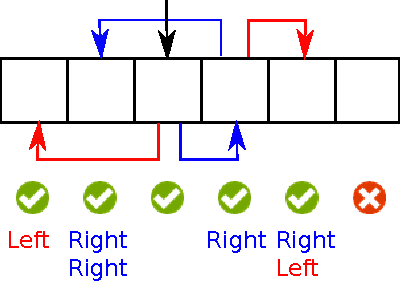
\includegraphics[width=5cm]{model.pdf}
\caption{\label{fig-binary-mod-ex} Example of model of a binary tree.}
\end{center}
\end{figure}

Only valid binary trees are associated a model, that is, the model function
only works on trees for which the tree structure invariant holds. As a result,
we cannot use this model function inside the implemenation of binary tree,
for example to state in the invariant that all the nodes are reachable from the
root (there is no memory leak). However, as type invariants always hold outside
of data structures implementation, the path model can safely be used for any
binary tree in the implementation of search trees. In particular, we use it
in the invariant of search trees, which is given in Figure~\ref{fig-search-inv}.

\begin{figure}[ht]
\begin{small}
\begin{lstlisting}
(for all I in Index_Type =>
  (for all J in Index_Type =>
    (if Model (F, Root) (I).K
       and then Model (F, Root) (J).K
       and then Model (F, Root) (I).A < Model (F, Root) (J).A
     then (if Get (Model (F, Root) (J).A, Length (Model (F, Root) (I).A) + 1)
              = Left
           then Values (J) < Values (I)
           else Values (J) > Values (I)))))
\end{lstlisting}
\end{small}
\caption{\label{fig-search-inv} Type invariant of search trees.}
\end{figure}

The invariant of search trees states that the value stored in each node of the
tree is bigger than all the values stored in the subtree rooted at its left
child and smaller than all the values stored in the subtree rooted at its right
child. An example of values that would fit the tree from Figure~\ref{fig-binary}
is given in Figure~\ref{fig-search}. To express this invariant, we use the
model of the underlying binary tree. A value V is stored in the subtree rooted
at the right child of a node if the path leading to this value is a supersequence
of the path leading to V and the next element in the sequence is Right.

\begin{figure}[ht]
\begin{center}
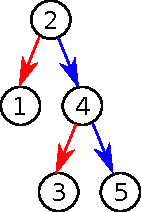
\includegraphics[width=2cm]{search.pdf}
\caption{\label{fig-search} Ordered nodes in a search tree.}
\end{center}
\end{figure}

Search trees are usually used to implement ordered sets. Though it is not needed to
specify the invariant of red black trees, we provide a model function returning the
set of all the values contained in the tree. We use it to annotate the insertion and
membership primitives provided on red black trees.

{\color{red} TODO: speak about red black trees}

\begin{figure}[ht]
\begin{center}
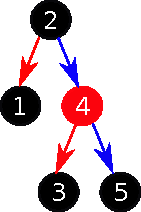
\includegraphics[width=2cm]{red_black.pdf}
\end{center}
\end{figure}

\subsection{Implementation}
% no pointer in spark => indexes inside an array
% avoid copies, use forest
% it is bounded
% values and colors are outside, in separate array (to avoid having them in the frame)
% provide plug/extract to modify the forest while keeping the invariant
% rotate_left and rotate_right preserve the order

From a software verification perspective, it may seem strange to present the implementation
before the specification. Here we do so because the implementation is comparatively
simpler and more widely known than the specification. And indeed, our implementation
resemble standard imperative implementations of red black trees except for to two notable
points. The first one is that we had to comply with the restrictions imposed by the
SPARK language, most notably, the forbidding of pointers (access types in Ada). To
alleviate this restriction, we chose to implement binary trees inside an array, indexes
working as pointers in a memory region. To simplify our implementation, we do not consider
node deallocation, so that unallocated cells are located after a given index in the array.
The Ada type of binary trees is given in Figure~\ref{fig-binary-typ}.
Note that our trees are bounded by the size of the underlying array.

\begin{figure}[ht]
\begin{small}
\begin{lstlisting}
type Cell is record
   Left, Right, Parent : Extended_Index_Type := Empty;
   Position            : Position_Type := Top;
end record;
type Cell_Array is array (Index_Type) of Cell;

type Forest is record
   S : Extended_Index_Type := Empty;
   C : Cell_Array;
end record
  with Type_Invariant => Tree_Structure (Forest);
--  Component S gives the size of the forest. Only the cells up to
--  index S belong to the forest. Cells after index S are free.
\end{lstlisting}
\end{small}
\caption{\label{fig-binary-typ} Implementation of binary trees.}
\end{figure}

The other specificity of our implementation is of course the layered design. Since we
have chosen to associate a type invariant to binary trees, the Forest type is defined as
a private type and it can only be modified by users using functions which abide by the
invariant. Therefore, we cannot change the values of the Cell record components individually
from outside of binary trees implementation. We have resorted to defining functions
doing single modifications of the tree while preserving the invariant. The modification
functions provided for binary trees are given in Figure~\ref{fig-binary-fun}.

\begin{figure}[ht]
\begin{small}
\begin{lstlisting}
function Parent (F : Forest; I : Index_Type)
    return Extended_Index_Type;
--  Parent in the tree structure

function Position (F : Forest; I : Index_Type) return Direction;
--  Position (Left or Right) in the tree structure

function Peek (F : Forest; I : Index_Type; D : Direction)
    return Extended_Index_Type;
--  Left or right child in the tree structure

procedure Init (F : in out Forest; Root : out Index_Type);
--  Initialize a new tree in F

procedure Extract (F       : in out Forest;
                   Root, I : Index_Type;
                   D       : Direction;
                   V       : out Extended_Index_Type);
--  Extract the subtree starting at position D after I in the tree
--  rooted at root in a separate tree. Store its root into V.

procedure Plug (F       : in out Forest;
                Root, I : Index_Type;
                D       : Direction;
                V       : Extended_Index_Type);
--  Plug the tree rooted at V in F into the tree rooted at Root as
--  a subtree starting at position D after I.

procedure Insert (F       : in out Forest;
                  Root, I : Index_Type;
                  D       : Direction;
                  V       : out Index_Type);
--  Insert a new node in F into the tree rooted at Root at position
--  D after node I. This is equivalent to calling succesively Init
--  and Plug.
\end{lstlisting}
\end{small}
\caption{\label{fig-binary-fun} Functions on binary trees.}
\end{figure}

Note that we are dealing everywhere with forests of binary trees instead of a single
binary tree. This is because, as we are using arrays instead of pointers, we cannot divide a
tree object into separate objects without copying the array arround. To keep an efficient
implementation, we resorted to processing the memory region as a whole, therefore
introducing forests of trees, in which every allocated node with a Top position is a
valid root.

As type invariants can be temporarily broken inside the data structure implementation, the body
of the modification functions can directly modify the internal structure of the tree. The implementation
of Plug is presented in Figure~\ref{fig-binary-body}.

\begin{figure}[ht]
\begin{small}
\begin{lstlisting}
procedure Plug (F       : in out Forest;
                Root, I : Index_Type;
                D       : Direction;
                V       : Extended_Index_Type) is
begin
   if V /= Empty then
      if D = Left then
         F.C (I).Left := V;
      else
         F.C (I).Right := V;
      end if;

      F.C (V).Position := D;
      F.C (V).Parent := I;
   end if;
end Plug;
\end{lstlisting}
\end{small}
\caption{\label{fig-binary-body} Implementation of Plug.}
\end{figure}

Following our leveled approach, search trees are defined outside of binary tree implementation.
They are binary trees along with an additional array of values. Also, as we never need to consider
parts of search trees, we no longer work on complete forests but rather on a single tree. More
precisely, we store a single root index in the search tree data structure.
The Ada type of search trees is given in Figure~\ref{fig-search-typ}.

\begin{figure}[ht]
\begin{small}
\begin{lstlisting}
type Value_Array is array (Index_Type) of Natural;

type Search_Tree is record
   Root   : Extended_Index_Type := Empty;
   Struct : Forest;
   Values : Value_Array := (others => 0);
end record
  with Type_Invariant => ...;
\end{lstlisting}
\end{small}
\caption{\label{fig-search-typ} Implementation of search trees.}
\end{figure}

The functions provided on search trees are basic set functions, namely inserting a value into the tree
and testing a value for membership into the tree. To allow implementation of red black trees above
search trees, balancing functions are also provided. Defining them inside the implementation of
search trees rather than inside the implementation of red black tree allow to keep all order-related
concerns in the search tree layer. Indeed, balancing functions do not preserve balancing, as they
are to be called on unbalanced trees, but they do preserve order. Note that implementing the balancing
functions at this level avoids the need for lifting low level tree handling functions such as Plug and
Extract. All the functions defined on search trees are implemented using
functions over binary forests. The functions provided for search trees are given in
Figure~\ref{fig-search-fun}. We only give the implementation of Right\_Rotate as an
example.

\begin{figure}
\begin{small}
\begin{lstlisting}
function Mem (T : Search_Tree; V : Natural) return Boolean;
--  Test for membership of V in T

procedure Insert
  (T : in out Search_Tree; V : Natural; I : out Extended_Index_Type);
--  Insert V in T. I is the new allocated node.

procedure Left_Rotate (T : in out Search_Tree; I : Index_Type);
--  Rotate the subtree rooted at I in T to the left

procedure Right_Rotate (T : in out Search_Tree; I : Index_Type) is
   X, Y    : Index_Type;
   XR      : Extended_Index_Type;
   Is_Root : constant Boolean := I = Root (T);
   P       : Index_Type;
   D       : Direction;

begin
   --  Y is the subtree located at I. Extract it as a separate tree.
   --  If Y is not a root, P is its parent.

   if Is_Root then
      Y := T.Root;
   else
      P := Parent (T.Struct, I);
      D := Position (T.Struct, I);
      Extract (T.Struct, T.Root, P, D, Y);
   end if;

   --  X is the left subtree of Y. Extract it as a separate tree.

   Extract (T.Struct, Y, Y, Left, X);

   --  XR is the right subtree of X. Extract it as a separate tree.

   Extract (T.Struct, X, X, Right, XR);

   --  Plug XR as the left subtree of Y

   Plug (T.Struct, Y, Y, Left, XR);

   --  Plug Y as the right subtree of X

   Plug (T.Struct, X, X, Right, Y);

   --  X takes the place of Y in the tree

   if Is_Root then
      T.Root := X;
   else
      Plug (T.Struct, T.Root, P, D, X);
   end if;
end Right_Rotate;
\end{lstlisting}
\end{small}
\caption{\label{fig-search-fun} Functions on binary trees.}
\end{figure}

Red black trees are implemented in the same way as search trees by adding an array of
colors to a search tree and using balancing functions to rebalance the tree after an insertion.

\subsection{Specification}
% use parent/position and model
% model can be derived from parent and position but have it in post to do inductive proofs only once
% invariant about no memory leak derived from post
% - of binary trees: we never have ill formed cyclic trees
% - of search trees: all cells remain accessible from the root

In this example, we concentrate on functional requirements of two kinds. The most important one is the
preservation of the data structure invariants. As a proof of concept, we have also considered
function specific requirements, describing the effect of the insertion and membership functions with
respect to the set of values contained in the red black tree. The function specific requirements are the
simplest. They are expressed as contracts on the tree functions. The set of values contains in a red black
tree is accessed using the appropriate model function. These contracts are presented in
Figure~\ref{fig-rbt-spec}.

\begin{figure}[ht]
\begin{small}
\begin{lstlisting}
function Values (T : Rbt) return Value_Set with
  Post => (if Size (T) = 0 then Is_Empty (Values'Result));

function Mem (T : Rbt; V : Natural) return Boolean with
  Post => Mem'Result = Mem (Values (T), V);

procedure Insert (T : in out Rbt; V : Natural) with
  Pre  => Size (T) < Max,
  Post => (if Mem (T'Old, V) then Values (T) = Values (T'Old)
           else Is_Add (Values (T'Old), V, Values (T)));
\end{lstlisting}
\end{small}
\caption{\label{fig-rbt-spec} Specification of red black trees.}
\end{figure}

Let us now consider the requirements dealing with data struture invariants.

\begin{enumerate}
 \item A red black tree is always a valid binary tree (we can navigate it from the root using Peek, Parent,
 and Position in the expected way).
 \item There is no memory leak (if we have inserted less than Max elements, there is still room enough in the
 data structure to insert a new element).
 \item The values stored in the tree are ordered (it is a valid search tree).
 \item The tree stays balanced (we only verify part of it, that is, that red nodes can only have black children).
\end{enumerate}

The specification of these invariants is not grouped in one point but rather separated at between the various levels,
so that every part is expressed at the place were it can be most naturally expressed. The first requirement is
enforced at the binary tree level. The tree structure invariant (see Section~\ref{sec-rbt-inv}),
ensures that the various cell components (Parent, Position, Left, and Right) are consistent. This is not enough
to ensure that all the allocated nodes in the forest belong to well-formed binary trees though, as it does
not rule out degenerated, root-less, cyclic structures that would arise from linking the root of a binary tree as the
child of one of its leafs. Still, this is enough to ensure that red black trees are always well formed, as red black
trees always have a specified root. Note that the fact that every node in the forest is part of
a well formed binary tree is ensured at the level of binary trees by enforcing that such degenerated structures can
never be created in the contracts of the data structure modification functions.

As a the level of binary trees we are dealing with forests, the second requirement is rather enforced at the level of
search trees. It is specified as a postcondition of every modification function of the search tree level.
Figure~\ref{fig-spec-no-leak} shows the part of the postcondtion of Right\_Rotate ensuring that it hasn't introduced
any dangling node. It uses the model function Model described in Section~\ref{sec-rbt-inv} to reason about reachability
in the tree structure.

\begin{figure}[ht]
\begin{small}
\begin{lstlisting}
procedure Right_Rotate (T : in out Search_Tree; I : Index_Type) with
  Post =>
    --  The size of the tree is preserved
    Size (T) = Size (T)'Old

    --  Nodes in the tree are preserved
    and then (for all J in Index_Type =>
               (if Model (T) (J).K then Model (T'Old) (J).K))
    and then (for all J in Index_Type =>
               (if Model (T'Old) (J).K then Model (T) (J).K));
\end{lstlisting}
\end{small}
\caption{\label{fig-spec-no-leak} Postcondition of Right\_Rotate dealing with abscence of memory leaks.}
\end{figure}

The third and fourth requirements are expressed in the type invariant of respectively search trees and red black trees
as explained in Section~\ref{sec-rbt-inv}.

But the functional requirements are not the only part of the specification. Indeed, as GNATprove works in a per
subprogram modular basis, specification also has to convey enough information, at each level, to verify not only the
requirements specified at this level, but also all the requirements specified at upper levels. For example, as
Right\_Rotate calls Plug and Extract, the specification of these functions need to provide enough information to
verify both the absence of memory leaks as stated in the postcondition of Right\_Rotate, but also the preservation of
the order of values, as stated in search trees invariant. The postcondition of Plug is given in
Figure~\ref{fig-spec-binary}.

\begin{figure}
\begin{small}
\begin{lstlisting}
procedure Plug (F       : in out Forest;
                Root, I : Index_Type;
                D       : Direction;
                V       : Extended_Index_Type)
   --  Plug the tree rooted at V in F into the tree rooted at Root as a subtree
   --  starting at position D after I.

with
  Pre =>
    --  Root is the root of a tree
    Valid_Root (F, Root)

    --  I is a node in this tree
    and then Model (F, Root) (I).K

    --  I has no child for direction D
    and then Peek (F, I, D) = Empty

    --  Root and V are different nodes
    and then Root /= V

    --  V is either empty or the root of a tree
    and then (if V /= Empty then Valid_Root (F, V)),
  Post =>
    --  The size of the forest does not change
    Size (F) = Size (F'Old)

    --  V is inserted in the tree as child D of I
    and then V = Peek (F, I, D)

    --  Except for V, roots are preserved
    and then (for all J in Index_Type =>
               (if Valid_Root (F'Old, J) and then J /= V then Valid_Root (F, J)))
    and then (for all J in Index_Type =>
               (if Valid_Root (F, J) then Valid_Root (F'Old, J)))

    --  Except for V, the value of parent link is preserved
    and then (for all J in Index_Type =>
               (if J /= V
                then Parent (F, J) = Parent (F'Old, J)))

    --  Except for V, the value of position is preserved for nodes which have
    --  a parent.
    and then (for all J in Index_Type =>
               (if J /= V and Parent (F, J) /= Empty
                then Position (F, J) = Position (F'Old, J)))

    --  Except at I for child D, all other children are preserved
    and then (for all J in Index_Type =>
               (for all E in Direction =>
                 (if J /= I or else E /= D
                  then Peek (F, J, E) = Peek (F'Old, J, E))))

    --  Nodes previously in the tree rooted at Root are still in the tree
    --  rooted at Root.
    and then (for all J in Index_Type =>
               (if Model (F, Root)'Old (J).K then Model (F, Root) (J).K))

    --  Nodes previously in the tree rooted at V are now in the tree rooted
    --  at Root.
    and then (for all J in Index_Type =>
               (if V /= Empty and then Model (F'Old, V) (J).K
                then Model (F, Root) (J).K))

    --  Nodes in the tree rooted at Root come either from the tree previously
    --  rooted at Root, or for those nodes which have V on their path, from
    --  the tree previously rooted at V.
    and then (for all I in Index_Type =>
               (if Model (F, Root) (I).K
                then (if V /= Empty and then Model (F, Root) (V).A <= Model (F, Root) (I).A
                      then Model (F'Old, V) (I).K
                      else Model (F'Old, Root) (I).K)))

    --  Paths are preserved for nodes that were previously in the tree
    and then (for all J in Index_Type =>
               (if Model (F'Old, Root) (J).K
                then Model (F, Root) (J).A = Model (F'Old, Root) (J).A))

    --  The path for nodes in the tree previously rooted at V is obtained
    --  by concatenating the path from Root to V and the path from V to the
    --  node.
    and then (for all J in Index_Type =>
               (if V /= Empty and then Model (F'Old, V) (J).K
                then Is_Concat (Q => Model (F, Root) (V).A,
                                V => Model (F'Old, V) (J).A,
                                P => Model (F, Root) (J).A)))

    --  All other trees in the forest are preserved
    and then (for all T in Index_Type =>
               (if Valid_Root (F'Old, T) and then Root /= T and then V /= T
                then Model (F, T) = Model (F'Old, T)));
\end{lstlisting}
\end{small}
\caption{\label{fig-spec-binary} Contract of Plug.}
\end{figure}
{\color{red} TODO: find a way to make Figure~\ref{fig-spec-binary} fit in the page.}


The postcondition of Plug describes how it modifies the tree structure. Theoretically,
describing how Parent and Position fields are updated by the call should be enough to
describe the effect on the whole structure. Still, to avoid having to redo complex
proofs each time Plug is call, we choose to also describe the effect of the modification
of Peek, and, more importantly, Model. This allows to clearly separate concerns and allow
the implementation of search trees to only concentrate on order related issues.

\subsection{Proof Principles}
% principle of inductive proofs on size of path
% principles of dealing with the frame condition: unmodified trees in forest

% reachability requires proof by induction on the size of the path
%   This is done using loops and loop invariants
% order requires case split
%   This is done using if statements

Verifying our red balck tree implementation has proved to be challenging, and above the
purely automatic capacity of the GNATprove tool. There are several reasons for this:

\begin{itemize}
 \item The imperative, pointer based implementation of red black trees makes it difficult
 to reson about disjointness of different trees/subtrees in the forest.
 \item Reasoning about reachability involves inductive proofs, which automatic provers are
 notoriously bad at.
 \item Reasoning about ordering involves using transitivity relations, that is, coming up with
 an intermediate value to consider, which usually eludes automatic provers.
 \item The size of the formulas to verified, number of verification conditions, and number of
 paths in the program are important enough to defy provers scalabiity.
\end{itemize}

To work around these limitations, we resorted to using auto-active verification techniques, which,
as described in Section~\ref{sec-prelim-auto-active}, allow to guide automatic provers without
resorting to a proof assistant. We explain some of these techniques in this section.

\paragraph{Intermediate lemmas:}
One of the most classical technique in manual proof consists in factoring some usefull
part of a proof in an intermediate lemma so that it can be verified independently and
use as many time as necessary. In auto-active verification, this can be done by introducing
a procedure with no output, which, when called, will cause the deductive engine to verify
its precondition and assume its postcondition. In Figure~\ref{fig-proof-lem}, we show an
intermediate lemma which can be used to verify that two trees of a single forest with different
roots are disjoint. A caller of this function will have to verify the T1 and T2 are different
valid root in F and get for free that there can be no node reachable from both roots in F.
Naturally, the lemma is not assumed, its actual proof is done when verifying the procedure
Prove\_Model\_Distinct.

\begin{figure}
\begin{small}
\begin{lstlisting}
procedure Prove_Model_Distinct (F : Forest; T1, T2 : Index_Type) with
--  Trees rooted at different indexes in the forest are disjoint.

  Pre  => T1 /= T2
    and then Valid_Root (F, T1)
    and then Valid_Root (F, T2),
  Post => (for all I in Index_Type =>
            (not Model (F, T1) (I).K or not Model (F, T2) (I).K));
\end{lstlisting}
\end{small}
\caption{\label{fig-proof-lem} Intermediate lemma stating disjointness of trees in a forest.}
\end{figure}

\paragraph{Reasoning by induction:}
Though some automatic provers are in fact able of doing simple inductive proofs, inductive reasoning
still most of the time requires manual interaction. In auto-active style, an inductive proof can be done
using loop annotations named loop invariants. In SPARK, loop invariants are normal assertions occuring in
loop statements but which are handled in an inductive way by GNATprove. Namely, the prover splits its
verification in two parts. First, it verifies that the invariant holds in the first iteration of the
loop and then that it holds in any following iteration knowing that it held in the previous one.
This behavior is exactly what we want for a proof by induction. For example, Figure~\ref{fig-proof-ind}
demonstrates how the intermediate lemma presented in Figure~\ref{fig-proof-lem} can be verified
using a loop to perform an induction over the size of the path from the T1 to any node reachable
from T1 in F. The loop goes from 1 to the maximum size of any branch in the forest F. As an
invariant, we have written the property we wanted to prove. To verify this procedure, GNATprove will
first check that the invariant holds in the first iteration of the loop, that is, that T1 itself cannot
be reached from T2. Then, it will proceed by induction to show that this holds for any node reachable
from T1 in F.

\begin{figure}
\begin{small}
\begin{lstlisting}
procedure Prove_Model_Distinct (F : Forest; T1, T2 : Index_Type) is
begin
   for N in Index_Type loop
      pragma Loop_Invariant
        (for all I in Index_Type =>
          (if Model (F, T1) (I).K and Length (Model (F, T1) (I).A) < N
           then not Model (F, T2) (I).K));
   end loop;
end Prove_Model_Distinct;
\end{lstlisting}
\end{small}
\caption{\label{fig-proof-ind} Proof by induction over the length of the path from the root to a node in the tree.}
\end{figure}

\paragraph{Case analysis}
As the number of cases to consider can sometimes confuse the prover, it is often usefull to split the
problem in a sensible way. A proof by case analysis is nothing more than an if statement, each branch
narrowing the cases to consider and possibly providing additional informations on how to carry out
the proof in this particular case. Figure~\ref{fig-proof-ca} shows how case analysis was used to
prove how tree models are modified by an application of Plug. It is divided in two cases: either
the node was already reachable from the actual root and then its model is unchanged, or it was reachable
from the plugged root, in which case the path leading to it from the new root is the path leading to
the plugged root in the new tree concatenated with the path leading from the plugged root to the node
in the old tree. 

\begin{figure}
\begin{small}
\begin{lstlisting}
--  Nodes have the same path in F_Old and F, or for those nodes
--  for which V is on the path, their path is obtained by
--  concatenating the path from Root to V and the path from V to
--  the node.
for KI in Index_Type loop

   --  Case 1: node KI is in the tree rooted at Root in F_Old. Use
   --  Preserve_Equal to prove the property for node KI, based on
   --  the knowledge that it holds for the parent of node KI.

   if Model (F, Root) (KI).K
     and then Length (Model (F, Root) (KI).A) = N
     and then Model (F_Old, Root) (KI).K
   then
      Preserve_Equal (S1 => Model (F, Root) (F.C (KI).Parent).A,
                      S2 => Model (F_Old, Root) (F.C (KI).Parent).A,
                      S3 => Model (F, Root) (KI).A,
                      S4 => Model (F_Old, Root) (KI).A,
                      D  => F.C (KI).Position);
   end if;

   --  Case 2: node KI is in the tree rooted at V in F_Old. Use
   --  Preserve_Concat to prove the property for node KI, based
   --  on the knowledge that it holds for the parent of node KI.

   if Model (F, Root) (KI).K
     and then Length (Model (F, Root) (KI).A) = N
     and then Model (F_Old, V) (KI).K
     and then KI /= V
   then
      Preserve_Concat (S1 => Model (F_Old, V) (F.C (KI).Parent).A,
                       S2 => Model (F, Root) (F.C (KI).Parent).A,
                       S3 => Model (F_Old, V) (KI).A,
                       S4 => Model (F, Root) (KI).A,
                       T  => Model (F, Root) (V).A,
                       D  => F.C (KI).Position);
   end if;

   --  Accumulate the knowledge that the property holds up to node
   --  KI.

   pragma Loop_Invariant
     (for all I in 1 .. KI =>
       (if Model (F, Root) (I).K and then Length (Model (F, Root) (I).A) <= N then
          (if Model (F_Old, Root) (I).K then Model (F, Root) (I).A = Model (F_Old, Root) (I).A)));
   pragma Loop_Invariant
     (for all I in 1 .. KI =>
       (if Model (F, Root) (I).K and then Length (Model (F, Root) (I).A) <= N then
         (if Model (F_Old, V) (I).K then
            Is_Concat (Q => Model (F, Root) (V).A,
                       V => Model (F_Old, V) (I).A,
                       P => Model (F, Root) (I).A))));
end loop;
\end{lstlisting}
\end{small}
\caption{\label{fig-proof-ca} Proof by case analysis of the effect of Plug on models.}
\end{figure}

Note that, to prove each cases, we use an intermediate lemma by calling the associated procedure.
Also note that, to be able to apply this reasoning on every node of the memory array, the case
analysis had to be enclosed in a loop. As GNATprove cannot accumulated knowledge without a loop
invariant, we had to restate everything tha was proved so far in the loop as a loop invariant.
Also note that this reasoning is a part of a reasoning by induction over the size of the path
leading to the node in the new tree, which is why we aready know the proposition holds for the
node's parent.

\paragraph{Guiding the proof}
There are other useful ways to guide the proof engine.

\begin{figure}
\begin{small}
\begin{lstlisting}
procedure Prove_Order_Total (T : Search_Tree; L : Index_Type; V : Natural)
   with
     Ghost,
     Global => null,
     Pre  =>
       --  The tree is not empty
       Size (T.Struct) > 0

       --  Repeat relevant parts of the search tree invariant
       and then T.Root /= Empty
       and then Valid_Root (T.Struct, T.Root)
       and then Ordered_Leafs (T.Struct, T.Root, T.Values)

       --  V is not found at the leaf
       and then T.Values (L) /= V

       --  The leaf L is in the tree, and does not have the correct child for
       --  continuing the search for V.
       and then Model (T.Struct, T.Root) (L).K
       and then (if V < T.Values (L) then Peek (T.Struct, L, Left) = Empty
                 else Peek (T.Struct, L, Right) = Empty)

       --  V is less than all the left ancestors up to L and greater than all
       --  the right ancestors up to L.
       and then (for all I in Index_Type =>
                  (if Model (T.Struct, T.Root) (I).K then
                    (if Model (T.Struct, T.Root) (I).A < Model (T.Struct, T.Root) (L).A
                     then (if Get (Model (T.Struct, T.Root) (L).A, Length (Model (T.Struct, T.Root) (I).A) + 1) = Left
                           then V < T.Values (I)
                           else V > T.Values (I))))),
     Post =>
       (for all I in Index_Type =>
         (if Model (T.Struct, T.Root) (I).K then T.Values (I) /= V))
   is
   begin
      --  Case 1: given a node I which does not have L on its path, consider
      --  the common ancestor of L and I returned by Find_Root. Instantiating
      --  Ordered_Leafs once with this common ancestor and L, and another time
      --  with this common ancestor and I, allows to prove that V cannot be the
      --  same as the value at I.
      pragma Assert
        (for all I in Index_Type =>
          (if Model (T.Struct, T.Root) (I).K
           then Model (T.Struct, T.Root) (Find_Root (T.Struct, T.Root, I, L)).K));

      --  Case 2: given a node I which has L on its path, use Prove_Model_Total
      --  to prove that it is necessarily on the other side of where V would be
      --  found.

      if V < T.Values (L) then
         Prove_Model_Total (T.Struct, T.Root, L, Left);
      else
         Prove_Model_Total (T.Struct, T.Root, L, Right);
      end if;
      pragma Assert
        (for all I in Index_Type =>
           (if Model (T.Struct, T.Root) (I).K
            and then Find_Root (T.Struct, T.Root, I, L) = L
            then T.Values (I) /= V));
   end Prove_Order_Total;
\end{lstlisting}
\end{small}
\caption{\label{fig-proof-guide} Guide the proof to show that if V has not been found along the expected path in T, then it is not in T.}
\end{figure}

\subsection{Ghost Code}
% different uses of ghost code

% For specification purpose:
% - typically ghost functions used in contracts
% - can be interesting to execute as test oracles
% For verification purpose:
% - typically ghost procedures containing proofs by induction (loops), by case analysis...
% - no need to execute them, they do not bring anything
% No way to distinguish between both right now.

% factored out in ghost procedures to keep efficiency
% with or without contracts (inlining)

\section{Development and Verification Data}
% number of assertions, loc of ghost code, etc.
% data on automatic verification
% feedback from development and verification cycles

\section{Related Work}
\label{related-work}

\section{Conclusion}


\paragraph*{Acknowledgements}


\bibliographystyle{plain}
\bibliography{nfm_2017}

\end{document}
